\documentclass[a4paper,12pt]{article}

\usepackage{mystyle}
\usepackage{mygeome}

\graphicspath{ {images/} }


% https://tex.stackexchange.com/questions/32501/how-to-get-a-good-divisible-by-symbol
\DeclareRobustCommand{\divby}{%
  \mathrel{\vbox{\baselineskip.65ex\lineskiplimit0pt\hbox{.}\hbox{.}\hbox{.}}}%
}


\definecolor{light-cyan}{RGB}{0, 204, 204}
\definecolor{light-purple}{RGB}{138, 43, 226}


\author{Алексеев Василий}
\title{Семинар 1}
\date{1 сентября 2020}


\begin{document}
  \maketitle
  
  \tableofcontents

  \thispagestyle{empty}
  
  \newpage
  
  \pagenumbering{arabic}


  \section{Матрицы и определители $2$-го и $3$-го порядков}

  \subsection{Матрицы}

  Матрица $A$ размера $m \times n$:
  \[
    A = \begin{pmatrix}
      a_{11} & a_{12} & \ldots & a_{1n}\\
      a_{21} & a_{22} & \ldots & a_{2n}\\
      \vdots & \vdots & \ddots & \vdots\\
      a_{m1} & a_{m2} & \ldots & a_{mn}
    \end{pmatrix} \in \RR^{m \times n}
  \]
  
  
  \subsubsection{Операции с матрицами}
  
  \begin{definition}[Сложение матриц]
    Пусть $A, B \in \RR^{n \times n}$.
    Суммой $A \hm+ B$ называется матрица $C \hm\in \RR^{n \times n}$, такая что
    $c_{ij} \hm= a_{ij} + b_{ij}$, $i, j \hm= 1, \ldots, n$.
  \end{definition}
  
  \begin{definition}[Умножение матрицы на число]
    Пусть $A \in \RR^{n \times n}, \alpha \in \RR$.
    Произведением матрицы $A$ на число $\alpha$ называется матрица $C$, такая что
    $c_{ij} \hm= \alpha \cdot a_{ij}$, $i, j \hm= 1, \ldots, n$.
  \end{definition}
  
  \begin{remark}
    Матрицы $\RR^{n \times n}$ с введённой операцией сложения и умножения на числа из $\RR$ образуют линейное пространство\footnote{\href{https://en.wikipedia.org/wiki/Vector\_space}{wikipedia.org/wiki/Vector\_space}}:
    \begin{enumerate}
      \item $A + B = B + A$, $\forall A, B \in \RR^{n \times n}$ (коммутативность сложения).
      \item $A + (B + C) = (A + B) + C$, $\forall A, B, C \in \RR^{n \times n}$ (ассоциативность сложения).
      \item $\exists 0_{n\times n} \in \RR^{n \times n}: 0_{n\times n} + A = A$, $\forall A \hm\in \RR^{n \times n}$.
      \item $\forall A \in \RR^{n \times n} \exists {-A} \in \RR^{n \times n}: A + ({-A}) = 0_{n\times n}$.
      \item $\alpha (\beta A) = (\alpha \beta) A$, $\forall \alpha, \beta \in \RR$, $\forall A \hm\in \RR^{n \times n}$ (ассоциативность умножения на скаляр).
      \item $1 \cdot A = A$, $\forall A \in \RR^{n \times n}$.
      \item $(\alpha + \beta) A = \alpha A + \beta A$, $\forall \alpha, \beta \hm\in \RR$, $A \hm\in \RR^{n \times n}$ (дистрибутивность умножения матрицы на число относительно сложения чисел).
      \item $\alpha (A + B) = \alpha A + \alpha B$, $\forall \alpha \hm\in \RR$, $A, B \hm\in \RR^{n \times n}$ (дистрибутивность умножения матрицы на число относительно сложения матриц).
    \end{enumerate}
  \end{remark}
  
  \begin{definition}[Умножение матриц]
    Пусть $A \hm\in \RR^{m \times p}$, $B \hm\in \RR^{p \times n}$.
    Тогда матрица $C$ называется произведением матриц $A$ и $B$, если
    \[
      \left\{
        \begin{aligned}
          &c_{ij} = \sum_{k = 1}^p a_{ik} b_{kj}\\
          &1 \leq i \leq m\\
          &1 \leq j \leq n
        \end{aligned}
      \right.
    \]
    и обозначается $C \hm= AB$.
  \end{definition}

  \begin{figure}[h]
    \centering
    
    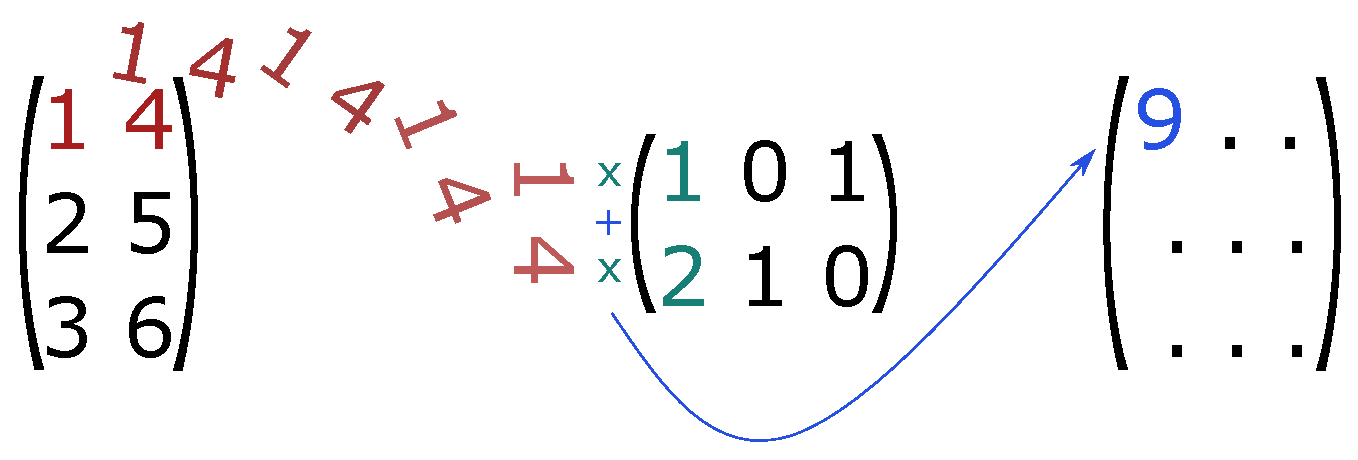
\includegraphics[width=0.5\columnwidth]{matrix-multiplication}
    
    \caption{Иллюстрация умножения матриц.}
    \label{fig:matrix-multiplication}
  \end{figure}
  
  \begin{problem}[15.5(7)]
    \[
      \begin{pmatrix}
        3 & 1\\
        2 & 1\\
        1 & 0
      \end{pmatrix}
      \begin{pmatrix}
        1 & 1\\
        1 & 1
      \end{pmatrix}= \?
    \]
  \end{problem}
  
  \begin{solution}
    \[
      \begin{pmatrix}
        3 & 1\\
        2 & 1\\
        1 & 0
      \end{pmatrix}
      \begin{pmatrix}
        1 & 1\\
        1 & 1
      \end{pmatrix}
      = \begin{pmatrix}
        3 \cdot 1 + 1 \cdot 1 & 3 \cdot 1 + 1 \cdot 1\\
        2 \cdot 1 + 1 \cdot 1 & 2 \cdot 1 + 1 \cdot 1\\
        1 \cdot 1 + 0 \cdot 1 & 1 \cdot 1 + 0 \cdot 1
      \end{pmatrix}
      = \begin{pmatrix}
        4 & 4\\
        3 & 3\\
        1 & 1
      \end{pmatrix}
    \]
  \end{solution}
  
  \begin{problem}[Т1$^*$]
    Для матриц $A, B, C$ определены произведения $AB, AC, BC$.
    Всегда ли определено произведение $BB \hm= B^2$?
  \end{problem}
  
  \begin{solution}
    Обозначим размерности (число строк и число столбцов) в матрицах $A, B, C$ за
    $(m_a, n_a),\ (m_b, n_b),\ (m_c, n_c)$ соответственно.
    Тогда условие задачи (возможность умножения матриц) можно переписать так:
    \[
      \left\{
        \begin{aligned}
          &m_a = n_b\\
          &m_a = n_c\\
          &m_b = n_c
        \end{aligned}
      \right.
    \]
    
    И получаем
    \[
      m_b = n_c = m_a = n_b \Rightarrow m_b = n_b
    \]
    
    Поэтому произведение $B^2$ также определено.
  \end{solution}
  
  \begin{problem}[15.11(9)]
    Вычислить матрицу в степени (произведение нескольких одинаковых матриц)
    \[
      \begin{pmatrix}
        0 & 1 & 0 & \ldots & 0\\
        0 & 0 & 1 & \ldots & 0\\
        \hdotsfor{5}\\
        0 & 0 & 0 & \ldots & 1\\
        1 & 0 & 0 & \ldots & 0
      \end{pmatrix}^n
    \]
  \end{problem}
  
  \begin{solution}
    Начинаем умножать и видим закономерность:
    \begin{equation*}
    \begin{split}
      \begin{pmatrix}
        0 & 1 & 0 & \ldots & 0\\
        0 & 0 & 1 & \ldots & 0\\
        \hdotsfor{5}\\
        0 & 0 & 0 & \ldots & 1\\
        1 & 0 & 0 & \ldots & 0
      \end{pmatrix}^n
      = &\begin{pmatrix}
        0 & 1 & 0 & \ldots & 0\\
        0 & 0 & 1 & \ldots & 0\\
        \hdotsfor{5}\\
        0 & 0 & 0 & \ldots & 1\\
        \textcolor{light-purple}{1} & 0 & 0 & \ldots & 0
        \end{pmatrix}
        \cdot \begin{pmatrix}
        0 & 1 & 0 & \ldots & 0\\
        0 & 0 & 1 & \ldots & 0\\
        \hdotsfor{5}\\
        0 & 0 & 0 & \ldots & 1\\
        1 & 0 & 0 & \ldots & 0
        \end{pmatrix}
        \cdot \begin{pmatrix}
          0 & 1 & 0 & \ldots & 0\\
          0 & 0 & 1 & \ldots & 0\\
          \hdotsfor{5}\\
          0 & 0 & 0 & \ldots & 1\\
          1 & 0 & 0 & \ldots & 0
        \end{pmatrix}^{n-2}\\
      = &\begin{pmatrix}
          0 & 0 & 1 & 0 & \ldots & 0\\
          0 & 0 & 0 & 1 & \ldots & 0\\
          \hdotsfor{6}\\
          0 & 0 & 0 & 0 & \ldots & 1\\
          \textcolor{light-purple}{1} & 0 & 0 & 0 & \ldots & 0\\
          0 & \textcolor{light-purple}{1} & 0 & 0 & \ldots & 0
        \end{pmatrix}
        \cdot \begin{pmatrix}
          0 & 1 & 0 & \ldots & 0\\
          0 & 0 & 1 & \ldots & 0\\
          \hdotsfor{5}\\
          0 & 0 & 0 & \ldots & 1\\
          1 & 0 & 0 & \ldots & 0
        \end{pmatrix}^{n-2}\\
      = &\begin{pmatrix}
          0 & 0 & 0 & 1 & \ldots & 0\\
          0 & 0 & 0 & 0 & \ldots & 0\\
          \hdotsfor{6}\\
          \textcolor{light-purple}{1} & 0 & 0 & 0 & \ldots & 0\\
          0 & \textcolor{light-purple}{1} & 0 & 0 & \ldots & 0\\
          0 & 0 & \textcolor{light-purple}{1} & 0 & \ldots & 0
        \end{pmatrix}
        \cdot \begin{pmatrix}
          0 & 1 & 0 & \ldots & 0\\
          0 & 0 & 1 & \ldots & 0\\
          \hdotsfor{5}\\
          0 & 0 & 0 & \ldots & 1\\
          1 & 0 & 0 & \ldots & 0
        \end{pmatrix}^{n-3}\\
      = &\begin{pmatrix}
          \textcolor{light-purple}{1} & 0 & 0 & \ldots & 0 & 0\\
          0 & \textcolor{light-purple}{1} & 0 & \ldots & 0 & 0\\
          0 & 0 & \textcolor{light-purple}{1} & \ldots & 0 & 0\\
          \vdots & \vdots & \vdots & \ddots & \vdots & \vdots\\
          \vdots & \vdots & \vdots & \ddots & \vdots & \vdots\\
          0 & 0 & 0 & \ldots & \textcolor{light-purple}{1} & 0\\
          0 & 0 & 0 & \ldots & 0 & \textcolor{light-purple}{1}
        \end{pmatrix}
        \cdot \begin{pmatrix}
          0 & 1 & 0 & \ldots & 0\\
          0 & 0 & 1 & \ldots & 0\\
          \hdotsfor{5}\\
          0 & 0 & 0 & \ldots & 1\\
          1 & 0 & 0 & \ldots & 0
        \end{pmatrix}^{n-n}
      = E_{n \times n}
    \end{split}
    \end{equation*}
  \end{solution}
  
  И ещё пара небесполезных концепций из мира матриц.
  
  \begin{definition}[Транспонирование матрицы]
    Пусть $A \in \RR^{n \times n}$.
    Тогда транспонированной по отношению к матрице $A$ матрицей называется такая матрица $С$, что
    $c_{ij} \hm= a_{ji}$.
    Транспонированная матрица обозначается $A^T$.
  \end{definition}
  
  \begin{definition}[След матрицы]
    Следом матрицы $A \in \RR^{n \times n}$ называется сумма элементов, находящихся на главной диагонали $\{a_{ij} \hm\mid i = j, i = 0, \ldots, n\}$:
    \[
      \left\{
        \begin{aligned}
          &\Sp \colon \RR^{n \times n} \to \RR\\
          &\Sp \colon A \mapsto \sum_{i = 1}^n a_{ii}
        \end{aligned}
      \right.
    \]
    У следа есть несколько возможных обозначений.
    Например, можно ещё писать $\Tr A$.
  \end{definition}


  \subsection{Определитель матрицы}
  
  Об определителе можно думать как о числовой функции на множестве матриц, обозначаемой $\det$ или $|\cdot|$
  \[
    \det \colon \RR^{n\times n} \to \RR
  \]
  и обладающей некоторыми свойствами.
  Конкретное определение $\det$ можно вводить по-разному (через свойства функции, или даже через конкретную формулу вычисления по элементам матрицы \ref{eq:complete-expansion}).
  Мы пока опустим строгое определение $\det$.
  Так как мы делаем фокус на решении задач, то нам не так важно последовательное изложение теории.
  Поэтому будем считать, что определитель ``просто есть'', как-то задан.
  И рассмотрим, как его вычислять для квадратных матриц размерности $2$, $3$, и пару свойств определителя (некоторые из которых следуют из определения, которое мы опускаем).
  
  \begin{example}
    Определитель второго порядка:
    \[
      \begin{vmatrix}
        a & b\\
        c & d
      \end{vmatrix} = ad - cb
    \]
  \end{example}

  \begin{example}
    Определитель третьего порядка (разложение по первой строке):
    \begin{equation*}
    \begin{split}
      &\begin{vmatrix}
        a_1 & b_1 & c_1\\
        a_2 & b_2 & c_2\\
        a_3 & b_3 & c_3
      \end{vmatrix}\\
        =\; &a_1 \cdot \begin{vmatrix}b_2 & c_2\\b_3 & c_3\end{vmatrix}
        - b_1 \cdot \begin{vmatrix}a_2 & c_2\\a_3 & c_3\end{vmatrix}
        + c_1 \cdot \begin{vmatrix}a_2 & b_2\\a_3 & b_3\end{vmatrix}\\
        =\; &a_1 b_2 c_3 - a_1 b_3 c_2 - a_2 b_1 c_3 + a_3 b_1 c_2 + a_2 b_3 c_1 - a_3 b_2 c_1
    \end{split}
    \end{equation*}
  \end{example}
  
  \begin{problem}[14.7(3)]
    \[
      \begin{pmatrix}
        1 & 2 & 2\\
        2 & 1 & -2\\
        2 & -2 & 1
      \end{pmatrix} = \?
    \]
  \end{problem}
  
  \begin{solution}
    \[
      \begin{pmatrix}
        1 & 2 & 2\\
        2 & 1 & -2\\
        2 & -2 & 1
      \end{pmatrix}
      = 1 \cdot \Bigl(1 \cdot 1 - (-2) \cdot (-2)\Bigr)
        \textcolor{light-cyan}{-} 2 \cdot \Bigl(2 \cdot 1 - 2 \cdot (-2)\Bigr)
        + 2 \cdot \Bigl(2 \cdot (-2) - 2 \cdot 1\Bigr)
      = -3 - 12 - 12
      = -27
    \]
  \end{solution}
  
  \begin{example}
    Определитель единичной матрицы:
    \[
      \det E = 1^n = 1
    \]
  \end{example}

  \begin{theorem}
    Определитель транспонированной матрицы
    \[
      \det A^T = \det A
    \]
  \end{theorem}
  
  \begin{theorem}
    Определитель произведения двух квадратных матриц:
    \[
      \det (AB) = \det A \cdot \det B
    \]
  \end{theorem}
  
  \begin{definition}[Вырожденная матрица\footnote{Определение вырожденной матрицы можно вводить по-разному. Ещё возможный вариант: квадратная матрица называется вырожденной, если её строки $\{\bds a_i\}_{i=1}^n$ линейно зависимы. Строки линейно зависимы~---~когда существует нетривиальная линейная комбинация строк, которая даёт нулевую строку: $\sum_{i=1}^n \alpha_i \bds a_i \hm= \bds 0$, $\sum_{i=1}^n \alpha_i^2 \hm > 0$.}]
    Матрица $A$ называется вырожденной, если $\det A \hm= 0$.
    В противном случае матрица $A$ называется невырожденной.
  \end{definition}
  
  \begin{theorem}
    Определитель обратной к \emph{невырожденной} матрице
    \[
      \det A^{-1} = \bigl(\det A\bigl)^{-1}
    \]
  \end{theorem}
  
  \begin{theorem}[Формула полного разложения определителя]\label{theor:complete-expansion}
    Пусть $A \in \RR^{n \times n}$.
    Тогда определитель $\det A$ матрицы равен
    \begin{equation}
      \label{eq:complete-expansion}
      \det A = \sum_{(i_1, \ldots, i_n)} (-1)^{N(i_1, \ldots, i_n)} a_{1 i_1} \ldots a_{n i_n}
    \end{equation}
    где $N(i_1, \ldots, i_n)$~---~число нарушений порядка в перестановке чисел $i_1, \ldots, i_n$\footnote{Нарушение порядка~---~когда правее большего элемента стоит меньший элемент: $i_k > i_s$, но $k < s$.}.
    Сумма в формуле берётся по всем перестановкам чисел $1, \ldots, n$\footnote{Например, перестановки чисел $1, 2, 3$: $(1, 2, 3), (1, 3, 2), (2, 1, 3), (2, 3, 1), (3, 1, 2), (3, 2, 1)$.}.
  \end{theorem}
  
  \begin{example}
    Вспомним формулу вычисления определителя для матрицы размера $3$:
    \begin{equation*}
      \begin{vmatrix}
        a_1 & b_1 & c_1\\
        a_2 & b_2 & c_2\\
        a_3 & b_3 & c_3
      \end{vmatrix}
        = a_1 b_2 c_3 - a_1 b_3 c_2 - a_2 b_1 c_3 + a_3 b_1 c_2 + a_2 b_3 c_1 - a_3 b_2 c_1
    \end{equation*}
    
    Элементы в каждом слагаемом упорядочены по номеру столбца.
    Поэтому посмотрим на число беспорядков по строкам (неважно, как считать беспорядки, по строкам или по столбцам, потому что $\det A \hm= \det A^T$).
    В первом слагаемом: $N(1, 2, 3) \hm= 0$.
    Во втором: $N(1, 3, 2) \hm= 1$ (тройка и двойка).
    В третьем: $N(2, 1, 3) \hm= 1$ (двойка и единица).
    В четвёртом: $N(3, 1, 2) \hm= 2$ (два беспорядка с тройкой и единицей и тройкой и двойкой).
    В пятом: $N(2, 3, 1) \hm= 1 \hm+ 1 \hm= 2$ (для двойки и единицы и для тройки и единицы).
    В шестом: $N(3, 2, 1) \hm= 2 \hm+ 1 \hm= 3$ (тройка-двойка, тройка-единица, двойка-единица).
  \end{example}
  
  
  \subsubsection{Свойства определителя}
  
  \begin{theorem}
    Некоторые свойства определителя (матрицы в формулах ниже представляются столбцами $\bds a_i \hm\in \RR^n$):
    \begin{enumerate}
      \item Линейность по столбцу (строке)~---~полилинейность:
        \[
          \left\{
            \begin{aligned}
              &\det (\bds a_1, \ldots, \underbrace{\bds p + \bds q}_{\bds a_i}, \ldots, \bds a_n)
                = \det (\bds a_1, \ldots, \bds p, \ldots, \bds a_n)
                + \det (\bds a_1, \ldots, \bds q, \ldots, \bds a_n)\\
              &\det (\bds a_1, \ldots, \underbrace{\alpha \bds p}_{\bds a_i}, \ldots, \bds a_n)
                = \alpha \det (\bds a_1, \ldots, \bds p, \ldots, \bds a_n)
            \end{aligned}
          \right.
        \]
      \item При перестановке двух столбцов (строк) матрицы её определитель меняет знак:
        \[
          \det (\bds a_1, \ldots, \bds a_{\textcolor{light-cyan}{i}}, \ldots, \bds a_{\textcolor{light-purple}{j}}, \ldots, \bds a_n)
          = -\det (\bds a_1, \ldots, \bds a_{\textcolor{light-purple}{j}}, \ldots, \bds a_{\textcolor{light-cyan}{i}}, \ldots, \bds a_n)
        \]
      \item Если два столбца (две строки) матрицы совпадают, то её определитель равен нулю:
        \[
          \det (\bds a_1, \ldots, \bds p, \ldots, \bds p, \ldots, \bds a_n) = 0
        \]
    \end{enumerate}
    
  \end{theorem}
  
  Свойства можно доказать как следствия теоремы \ref{theor:complete-expansion}.
  
  И ещё пара более частных утверждений, которые следуют/являются подслучаями свойств выше:
  \begin{itemize}
    \item Общий множитель элементов строки (столбца) можно выносить за знак определителя:
      \[
        \det (\bds a_1, \ldots, \alpha \bds p, \ldots, \bds a_n)
          = \alpha \cdot \det (\bds a_1, \ldots, \bds p, \ldots, \bds a_n)
      \]
    \item К любой строке (столбцу) матрицы можно прибавлять линейную комбинацию других строк (столбцов)~---~определитель при этом не изменится:
      \[
        \det (\bds a_1, \ldots, \bds a_i, \ldots, \bds a_n)
          = \det (\bds a_1, \ldots, \sum_{\substack{1 \leq j \leq n\\j \not= i}} \alpha_j \bds a_j + \bds a_i, \ldots, \bds a_n)
      \]
    \item При вычислении определителя матрицы вида $\alpha A$ скаляр $\alpha$ можно выносить за знак $\det$ следующим образом:
      \[
        \det \alpha A = \alpha^n \det A
      \]
  \end{itemize}
  
  \begin{problem}[14.24(1)]
    Вычислить определитель порядка $n$
    \[
      \begin{vmatrix}
        1 & 1 & 1 & \ldots & 1 & 1 & 1\\
        1 & 1 & 0 & \ldots & 0 & 0 & 0\\
        0 & 1 & 1 & \ldots & 0 & 0 & 0\\
        \hdotsfor{7}\\
        0 & 0 & 0 & \ldots & 1 & 1 & 0\\
        0 & 0 & 0 & \ldots & 0 & 1 & 1
      \end{vmatrix} = \?
    \]
  \end{problem}
  
  \begin{solution}
    Раскладываем определитель по первому столбцу:
    \[
      \begin{vmatrix}
        1 & 1 & 1 & \ldots & 1 & 1 & 1\\
        1 & 1 & 0 & \ldots & 0 & 0 & 0\\
        0 & 1 & 1 & \ldots & 0 & 0 & 0\\
        \hdotsfor{7}\\
        0 & 0 & 0 & \ldots & 1 & 1 & 0\\
        0 & 0 & 0 & \ldots & 0 & 1 & 1
      \end{vmatrix}
      = 1 \cdot \begin{vmatrix}
          1 & 0 & 0 & \ldots & 0 & 0 & 0\\
          1 & 1 & 0 & \ldots & 0 & 0 & 0\\
          0 & 1 & 1 & \ldots & 0 & 0 & 0\\
          \hdotsfor{7}\\
          0 & 0 & 0 & \ldots & 1 & 1 & 0\\
          0 & 0 & 0 & \ldots & 0 & 1 & 1
        \end{vmatrix}
        - 1 \cdot \begin{vmatrix}
          1 & 1 & 1 & \ldots & 1 & 1 & 1\\
          1 & 1 & 0 & \ldots & 0 & 0 & 0\\
          0 & 1 & 1 & \ldots & 0 & 0 & 0\\
          \hdotsfor{7}\\
          0 & 0 & 0 & \ldots & 1 & 1 & 0\\
          0 & 0 & 0 & \ldots & 0 & 1 & 1
        \end{vmatrix}
    \]
    
    Рассмотрим первый из определителей во второй части равенства выше.
    Пользуясь свойствами определителя, его можно посчитать так:
    \begin{equation*}
    \begin{split}
      \begin{vmatrix}
        1 & 0 & 0 & \ldots & 0 & 0 & 0\\
        1 & 1 & 0 & \ldots & 0 & 0 & 0\\
        0 & 1 & 1 & \ldots & 0 & 0 & 0\\
        \hdotsfor{7}\\
        0 & 0 & 0 & \ldots & 1 & 1 & 0\\
        0 & 0 & 0 & \ldots & 0 & 1 & 1
      \end{vmatrix}
      = &\begin{vmatrix}
          1 & 0 & 0 & \ldots & 0 & 0 & 0\\
          \textcolor{light-cyan}{0} & 1 & 0 & \ldots & 0 & 0 & 0\\
          0 & 1 & 1 & \ldots & 0 & 0 & 0\\
          \hdotsfor{7}\\
          0 & 0 & 0 & \ldots & 1 & 1 & 0\\
          0 & 0 & 0 & \ldots & 0 & 1 & 1
        \end{vmatrix}\\
      = &\begin{vmatrix}
          1 & 0 & 0 & \ldots & 0 & 0 & 0\\
          0 & 1 & 0 & \ldots & 0 & 0 & 0\\
          0 & \textcolor{light-cyan}{0} & 1 & \ldots & 0 & 0 & 0\\
          \hdotsfor{7}\\
          0 & 0 & 0 & \ldots & 1 & 1 & 0\\
          0 & 0 & 0 & \ldots & 0 & 1 & 1
        \end{vmatrix}
      = \ldots
      = \begin{vmatrix}
          1 & 0 & 0 & \ldots & 0 & 0 & 0\\
          0 & 1 & 0 & \ldots & 0 & 0 & 0\\
          0 & 0 & 1 & \ldots & 0 & 0 & 0\\
          \hdotsfor{7}\\
          0 & 0 & 0 & \ldots & 0 & 1 & 0\\
          0 & 0 & 0 & \ldots & 0 & 0 & 1
        \end{vmatrix}
      = 1^{n - 1}
      = 1
    \end{split}
    \end{equation*}
    
    Если обозначит искомый определитель как $\Delta_n$, то второй из определителей в первой формуле есть просто $\Delta_{n-1}$.
    Итого,
    \[
      \Delta_n = 1 - \Delta_{n-1}
    \]
    
    Посмотрим на $\Delta_n$ при $n \hm= 1, 2, \ldots$:
    \[
      \begin{aligned}
        &\Delta_1 = 1\\
        &\Delta_2 = 1 - 1 = 0\\
        &\Delta_3 = 1 - 0 = 1\\
        &\Delta_4 = 1 - 1 = 0\\
        &\Delta_5 = 1 - 0 = 1\\
        &\ldots
      \end{aligned}
    \]
    
    Очевидно\footnote{$a \divby p \equiv p \mid a$},
    \[
      \Delta_n = \left\{
        \begin{aligned}
          &1, 2 \not\mid n\\
          &0, 2 \mid n
        \end{aligned}
      \right.
      \equiv [2 \not\mid n]\footnote{Встречаются такие более короткие записи выражения индикатора (либо $0$, либо $1$ в зависимости от некоторого условия): $[\cdot]$, $I[\cdot]$. Например, ``$b$ равно $3$, если $a$ равно $2$; иначе $b$ равно $17.5$'' можно записать так: $b \hm= 3 \hm\cdot [a \hm= 2] + 17.5 \cdot [a \hm{\not=} 2]$.}
    \]
  \end{solution}
  

  \section{Системы линейныx уравнений. Правило Крамера}
  
  Система $m$ линейных уравнений с $n$ неизвестными:
  \[
    \renewcommand{\arraycolsep}{2pt}
    \left\{
      \begin{array}{lcl}
        a_{11} x_1 + \ldots + a_{1n} x_n & = & b_1\\
        \hdotsfor{3}\\
        a_{m1} x_1 + \ldots + a_{mn} x_n & = & b_n
      \end{array}
    \right.
  \]
  
  В матричном виде:
  \[
    \begin{pmatrix}
      a_{11} & \ldots & a_{1n}\\
      \vdots & \ddots & \vdots\\
      a_{m1} & \ldots & a_{mn}
    \end{pmatrix}
    \begin{pmatrix}
      x_1\\
      \vdots\\
      x_n
    \end{pmatrix}
    =
    \begin{pmatrix}
      b_1\\
      \vdots\\
      b_n
    \end{pmatrix}
  \]
  
  Или так:
  \[
    A \bds x = \bds b
  \]
  
  \begin{definition}[Решение системы]
    \[
      \{\bds x \in \RR^N \mid A \bds x = \bds b\}
    \]
  \end{definition}
  
  \begin{definition}
    Система называется совместной, если она имеет хотя бы одно решение, и несовместной, если у неё нет решений.
  \end{definition}
  
  \begin{definition}
    Говорят, что система $B$ следует из системы $A$, если множество решений $B$ содержит множество решений $A$ \ref{fig:a-and-b-sets}.
  \end{definition}
  
  \begin{figure}[h]
    \centering
    
    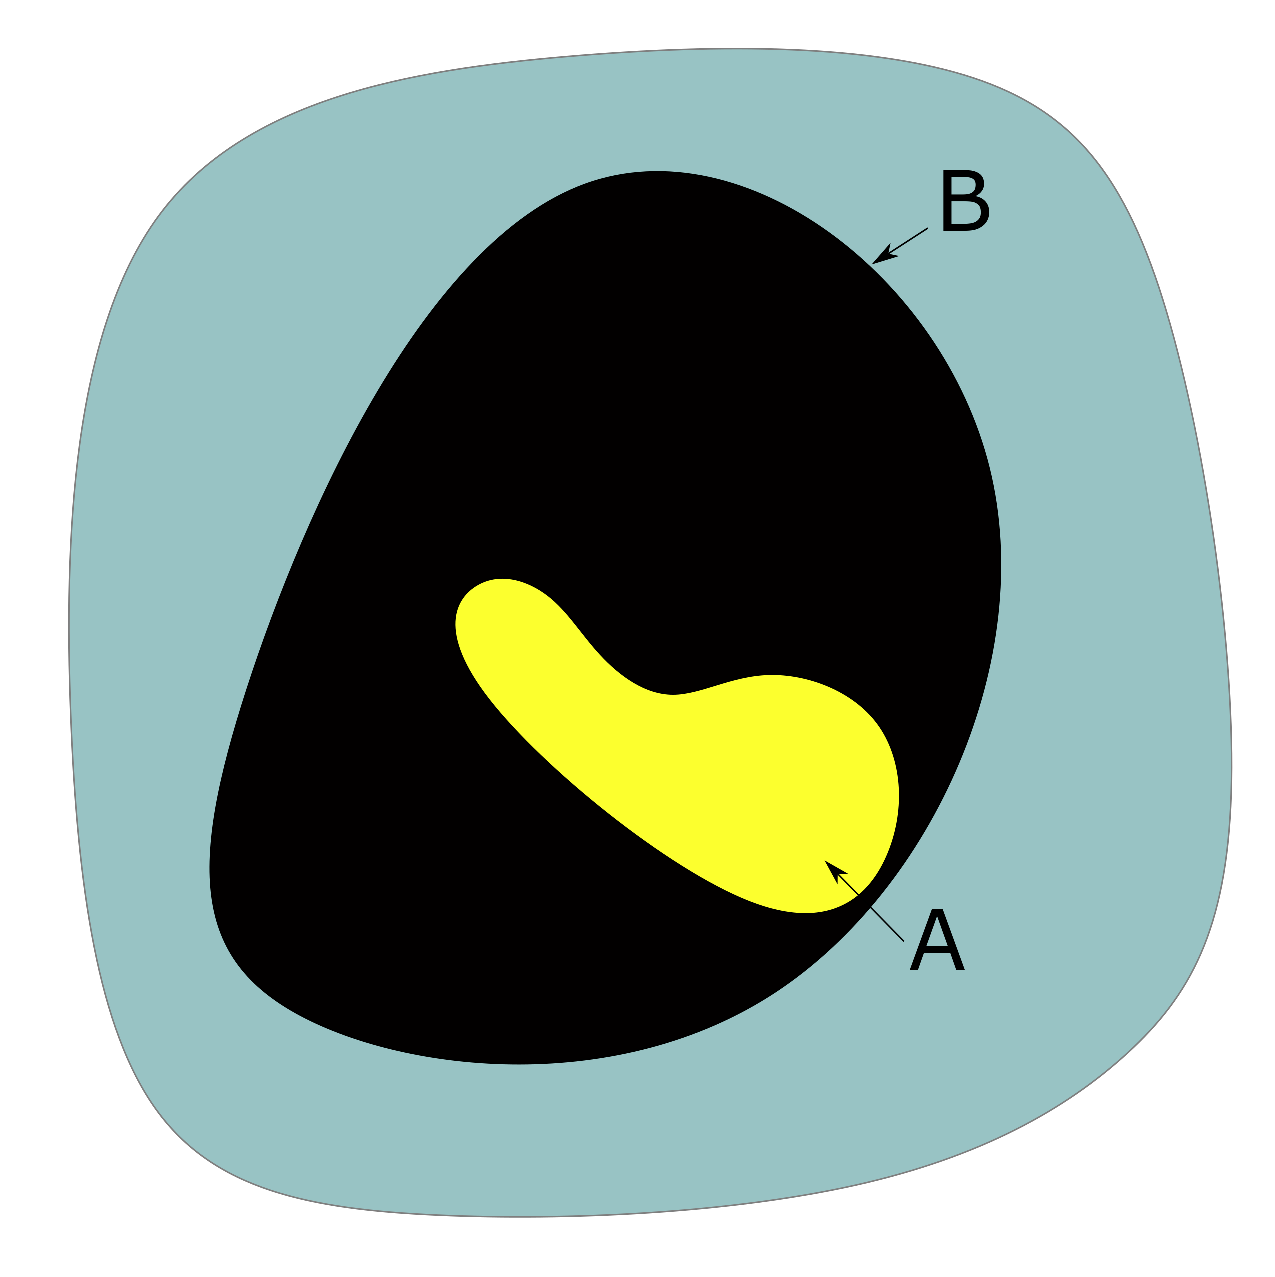
\includegraphics[width=0.5\columnwidth]{a-and-b-sets}
    
    \caption{Множество решений $A$ содержится во множестве решений $B$.}
    \label{fig:a-and-b-sets}
  \end{figure}
  
  \begin{theorem}
    Пусть число уравнений в системе $m$ равно числу неизвестных $n$.
    Тогда если $\det A \hm{\not=} 0$, то система $A \bds x \hm= \bds b$ имеет решение, и притом только одно.
  \end{theorem}
  
  \begin{theorem}[Правило Крамера]
    Пусть число уравнений в системе $m$ равно числу неизвестных $n$.
    Тогда если $\det A \hm{\not=} 0$, то
    \[
      \left\{
        \begin{aligned}
          &x_i = \frac{\Delta_i}{\Delta}\\
          &\Delta \equiv \det A\\
          &\Delta_i \equiv \det (\bds a_1, \ldots, \bds a_{i - 1}, \bds b, \bds a_{i + 1}, \ldots, \bds a_n)
        \end{aligned}
      \right.
    \]
  \end{theorem}
  
  \begin{problem}[17.2(4)]
    \[
      \left\{
        \begin{aligned}
          &A \bds x = \bds b\\
          &A = \begin{pmatrix}
            1 & -3 & -1\\
            -2 & 7 & 2\\
            3 & 2 & -4
          \end{pmatrix}\\
          &\bds b = \begin{pmatrix}
            -4\\ 10\\ 9
          \end{pmatrix}
        \end{aligned}
      \right.
    \]
  \end{problem}
  
  \begin{solution}
    \[
      \Delta = \det \begin{pmatrix}
        1 & -3 & -1\\
        -2 & 7 & 2\\
        3 & 2 & -4
      \end{pmatrix} = -1
    \]
    \[
      \Delta_1 = \det \begin{pmatrix}
        -4 & -3 & -1\\
        10 & 7 & 2\\
        9 & 2 & -4
      \end{pmatrix} = -3 \Rightarrow x_1 = \frac{\Delta_1}{\Delta} = \frac{-3}{-1} = 3
    \]
    \[
      \Delta_2 = \det \begin{pmatrix}
        1 & -4 & -1\\
        -2 & 10 & 2\\
        3 & 9 & -4
      \end{pmatrix} = -2 \Rightarrow x_2 = \frac{\Delta_2}{\Delta} = \frac{-2}{-1} = 2
    \]
    \[
      \Delta_3 = \det \begin{pmatrix}
        1 & -3 & -4\\
        -2 & 7 & 10\\
        3 & 2 & 9
      \end{pmatrix} = -1 \Rightarrow x_3 = \frac{\Delta_3}{\Delta} = \frac{-1}{-1} = 1
    \]
    \[
      \bds x = \begin{pmatrix}
        3\\ 2\\ 1
      \end{pmatrix}
    \]
  \end{solution}
  
\end{document}